\documentclass[a4paper, 11pt]{article}
\usepackage[pdftex]{graphicx}
\usepackage{parskip}
\usepackage{hyperref}
\usepackage[all]{hypcap}
\usepackage{amsmath}
\usepackage{amsfonts}
\usepackage{xcolor}
\usepackage{enumitem}
\usepackage{dsfont}
\title{Assignment 3 -- Math 205 Linear Algebra}
\author{Syed Ammar Mahdi \\sm03691 \and Muhammad Shahzain \\ms03977 \and Muhammad Shahrom Ali \\ma03559}

\newcommand{\mat}[1]{\boldsymbol { \mathsf{#1}} }
\newcommand{\MYhref}[3][blue]{\href{#2}{\color{#1}{#3}}}


\begin{document}
\setlength{\parskip}{10pt} % 1ex plus 0.5ex minus 0.2ex}
\setlength{\parindent}{0pt}
\DeclareGraphicsExtensions{.pdf,.png,.gif,.jpg}
\maketitle

\section*{Solutions}
\begin{enumerate} 

\item Does the following set of polynomials constitute a basis for subspace of polynomial of degree less than equal to 2 \[
\left\{x^2 + x + 1, x^2 - x + 1, 2x^2, 1 \right\}
\]

\textbf{Solution}

%Q1

Setting each vector as a row in a matrix

$
\begin{bmatrix} 
1 & 1 & 1 \\ 1 & -1 & 1 \\ 
2 & 0 & 0 \\ 0 & 0 & 1
\end{bmatrix}
$

Apply Gaussian elimination.

$R_1 + R_2$

$
\begin{bmatrix} 
1 & 1 & 1 \\ 2 & 0 & 2 \\ 
2 & 0 & 0 \\ 0 & 0 & 1
\end{bmatrix}
$

$-2R_4 + R_2$

$R_3 + R_2$

$
\begin{bmatrix} 
1 & 1 & 1 \\ 0 & 0 & 0 \\ 
2 & 0 & 0 \\ 0 & 0 & 1
\end{bmatrix}
$

Here we get a zero vector which shows that this set is not linearly independent. Hence, this set does not constitute a basis for subspace of polynomials of degree less than equal to 2. 

\item Find a basis for the space of polynomials $p(x)$ of degree $\leq 2$? Then, find the basis for the subspace with $p(7) = 0$ and sketch the bases.

\textbf{Solution}

%Q2

Any polynomial of $degree \leq 2$ can be represented as 

\begin{equation}
    p(x) = ax^2 + bx + c
\end{equation}{}

which can be represented as a linear combination of vectors $x^2, x,$  and $1$.

The vectors $\{ x^2, x, 1 \}$ is a basis for all polynomials with degree $\leq 2$. 

A linear combination of these bases will form a polynomial of degree 2 (Quadratic) if $a_1$ is non-zero. 

\begin{center}
    $p(x) = a_1x^2 + a_2x + a_31$
\end{center}

If only $a_1$ is zero, the polynomial is of degree 1 (Linear). 

\begin{center}
    $p(x) = 0.x^2 + a_2x + a_31$
    
    $p(x) = a_2x + a_31$
\end{center}

If both, $a_1$ and $a_2$ are zero, then the polynomial is degree 0(constant)

\begin{center}
    $p(x) = 0x^2 + 0x + a_31$
    
    $p(x) = a_3$

\end{center}

For a subspace with $p(7) = 0$, 

\begin{equation}
    p(7) = a(7)^2 + b(7) + c = 0
\end{equation}

\begin{center}
    $49a + 7b + c = 0$
    
    $c = -49a -7b$
    
    $p(x) = ax^2 + bx -49a -7b$
    
    $p(x) = ax^2 -49a + bx -7b$
    
    $p(x) = a(x^2 - 49) + b(x - 7)$
    
    basis = \{ $(x^2 -49)$, ($x -7)$ \}

    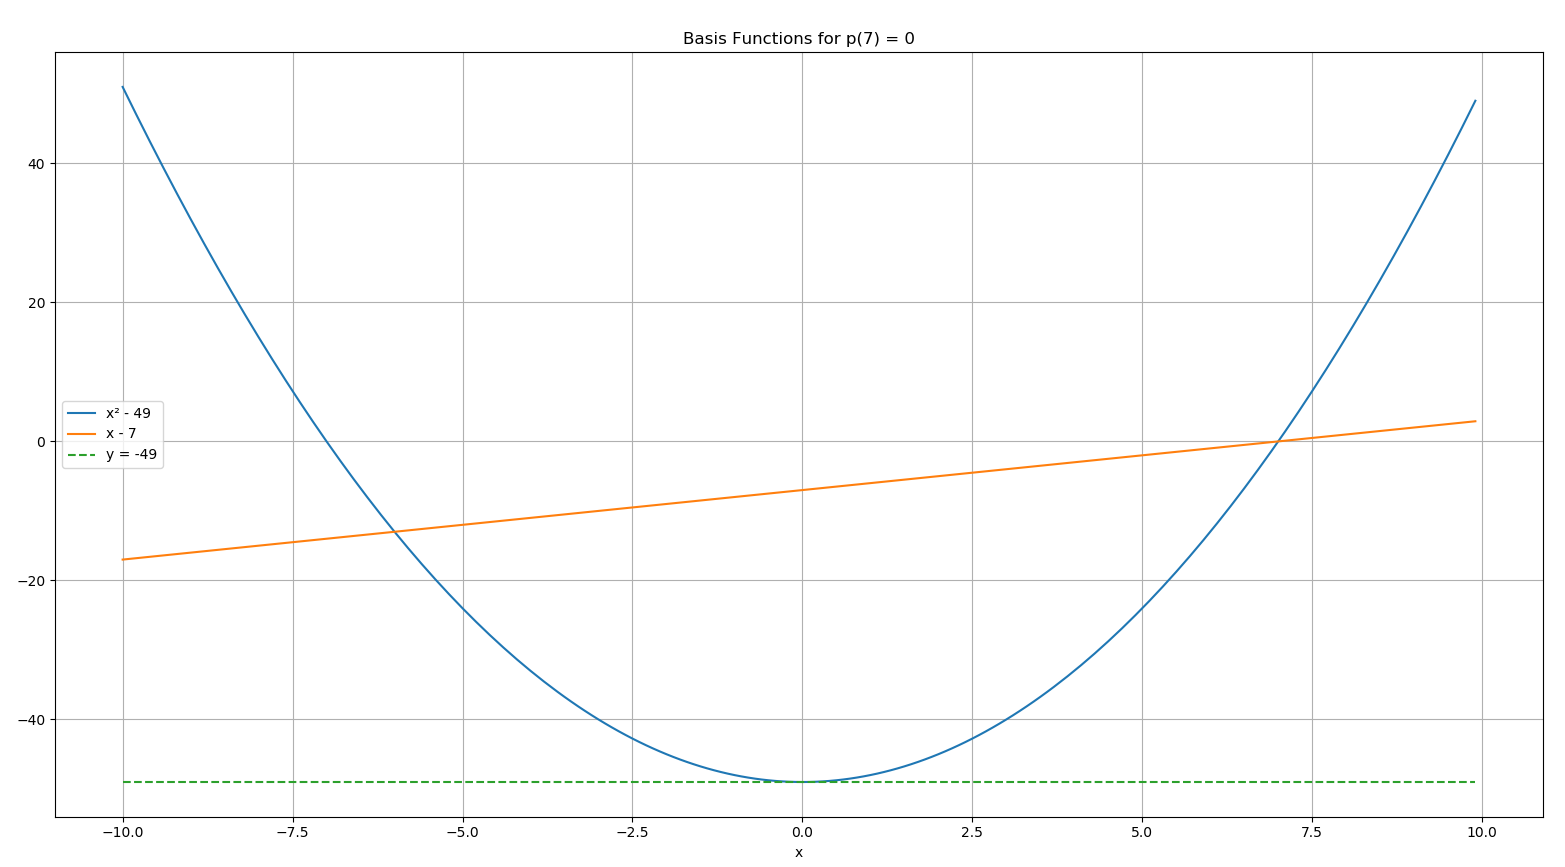
\includegraphics[width=\linewidth]{figs/Q2basis.png}
    Basis Sketch
\end{center}


\item Let $P_3$ be the real number vector space over $\mathbb R$ of cubic polynomials. $W$ is defined as \[
W = \{p(x) \in P_3 \;|\; p'(-1) = 0 \;\; \text{and} \;\; p''(1) = 0\}
\]

Determine whether $W$ forms a subspace of $V$

% Q3
\textbf{Solution:}

Form of all cubic polynomials:

\begin{equation}
	p(x) = ax^3 + bx^2 + cx + d
\end{equation}

Conditions: $p'(-1) = 0$ and $p''(1) = 0$

\begin{equation}
	p'(x) = 3ax^2 + 2bx + c
\end{equation}

\begin{center}
	$p'(-1) = 3a -2b + c = 0$

	$c = 2b - 3a$
\end{center}

\begin{equation}
	p''(x) = 6ax + 2b
\end{equation}

\begin{center}
	$p''(1) = 6a + 2b = 0$

	$b = -3a$

	$c = 2b - 3a$

	$c = -6a - 3a$

	$c = -9a$

	$a = -\frac{1}{9}c$

	$c = 3b$

	$b = \frac{1}{3}c$

\end{center}

The form of the cubic polynomials in $W$ then becomes

\begin{equation}
	p(x) = -\frac{1}{9}cx^3 + \frac{1}{3}cx^2 + cx + d
\end{equation}

$W$ contains all polynomials of this form.

Conditions for a valid subspace: 
\begin{enumerate}
	\item $p(x) + q(x) \in W$
	\item $a.p(x) \in W$ where $a \in \mathbb{R}$
\end{enumerate}

\begin{center}
	$p(x) = -\frac{1}{9}cx^3 + \frac{1}{3}cx^2 + cx + d$

	$q(x) = -\frac{1}{9}ax^3 + \frac{1}{3}ax^2 + ax + b$

	$r(x) = p(x) + q(x)$

	Check if $r(x) \in W$ 

	$r(x) = -\frac{1}{9}cx^3 + \frac{1}{3}cx^2 + cx + d + (-\frac{1}{9}ax^3 + \frac{1}{3}ax^2 + ax + b)$

	$r(x) = -\frac{1}{9}(c+a)x^3 + \frac{1}{3}(c+a)x^2 + (c + a)x + b + d$

	$r'(x) = -\frac{1}{3}(c+a)x^2 + \frac{2}{3}(c+a)x + c + a$
	
	$r'(-1) = -\frac{1}{3}(c + a) - \frac{2}{3}(c+a) + c + a$
	
	$r'(-1) = -\frac{3}{3}(c + a) + c + a$
	
	$\mathbf{r'(-1) = 0}$
	
	$r''(x) = -\frac{2}{3}(c + a)x + \frac{2}{3}(c+a)$
	
	$r''(1) = -\frac{2}{3}(c+a) + \frac{2}{3}(c+a)$
	
	$\mathbf{r''(1) = 0}$
	
	Condition (a) holds True.
	
	$q(x) = a.p(x)$ where $a \in \mathbb{R}$
	
	Check if $q(x) \in W$
	
	$q(x) = a.p(x) = a(-\frac{1}{9}cx^3 + \frac{1}{3}cx^2 + cx + d)$
	
	Since $a$ is just a constant, we know 
	
	$q'(x) = a.p'(x)$ 
	
	$q'(-1) = a.p'(-1)$
	
	$q'(-1) = a.0 = 0$
	
	$q''(x) = a.p''(x)$
	
	$q''(1) = a.p''(1)$
	
	$q''(1) = a.0 = 0$
	
	Condition (b) also holds.
	
	$W$ is closed under addition and multiplication, hence $W$ is a subspace of $V$.
\end{center}

% End of Q3

\item Find the bases for the four subspaces associated with $\mat A$ and $\mat B$:
\[ A = \left[ \begin{array}{ccc}
1&2&4\\
2&4&8
\end{array} \right]
\hspace{10mm}, B = \left[ \begin{array}{ccc}
1&2&4\\
2&5&8
\end{array} \right]\]
Sketch the four subspaces if an arbitrary matrix $\mat C$ is \begin{itemize}
  \item invertible
  \item a zero matrix
\end{itemize}

\textbf{Solution:}

C(A) = span\{ 
$\begin{bmatrix} 1 \\ 2 \end{bmatrix}$ \}

$\begin{bmatrix} 
1 & 2 & 4 \\ 2 & 4 & 8
\end{bmatrix}
\begin{bmatrix} 
x_1 \\ x_2 \\ x_3
\end{bmatrix}
 = 
 \begin{bmatrix}
 0 \\ 0 
\end{bmatrix}
$

$-2R_1 + R_2$

$\begin{bmatrix} 
1 & 2 & 4 \\ 0 & 0 & 0
\end{bmatrix}
\begin{bmatrix} 
x_1 \\ x_2 \\ x_3
\end{bmatrix}
 = 
 \begin{bmatrix}
 0 \\ 0 
\end{bmatrix}
$

$x_1 + 2x_2 + 4x_3 = 0$

$x_1 = -2x_2 - 4x_3$

$\begin{bmatrix} 
x_1 \\ x_2 \\ x_3
\end{bmatrix}$

$\begin{bmatrix} 
-2x_2 - 4x_3 \\ x_2 \\ x_3
\end{bmatrix}$

$\begin{bmatrix} 
-2x_2 \\ x_2 \\ 0
\end{bmatrix}
 +
\begin{bmatrix} 
-4x_3 \\ 0 \\ x_3
\end{bmatrix}
$

$x_2
\begin{bmatrix} 
-2 \\ 1 \\ 0
\end{bmatrix}
+
x_3
\begin{bmatrix} 
-4 \\ 0 \\ 1
\end{bmatrix}
$

N(A) = span\{
$\begin{bmatrix} 
-2 \\ 1 \\ 0
\end{bmatrix}
,
\begin{bmatrix} 
-4 \\ 0 \\ 1
\end{bmatrix}
$
\}


\item Find the complete solution for the following equations and describe the solution space:
\begin{equation} \label{eq1}
\begin{split}
x + 3y + 3z = 1 \\
2x + 6y + 9z = 5 \\
-x - 3y +3z =5 \\
\end{split}
\end{equation}

\textbf{Solution}

First, we rewrite the above system of equations as an augmented matrix $[\mat{A}|\textbf{b}]$:
\begin{equation*}
    \left(\begin{array}{ccc|c}  
    1 & 3 & 3 & 1 \\  
    2 & 6 & 9 & 5 \\
    -1 & -3 & 3 & 5 \\
    \end{array}\right)
\end{equation*}

Perform the following row operations to obtain the reduced row echelon form $\mat{R}$:

\begin{center}
    $R_{3} + R_{1}$ \\
    $-2R_{1} + R_{2}$ \\
    $-R_{2} + R_{1}$ \\
    $\frac{1}{3}R_{2}$ \\
    $\frac{1}{6}R_{3}$ \\
\end{center}

Which gives us the following augmented matrix:

\begin{equation*}
    \left(\begin{array}{ccc|c}  
    1 & 3 & 0 & -2 \\  
    0 & 0 & 1 & 1 \\
    0 & 0 & 0 & 0 \\
    \end{array}\right)
\end{equation*}

By looking at the left-hand-side of the augmented matrix above, i.e. $\mat{R}$, we can deduce that our matrix $\mat{A}$ has the rank $r = 2$. $r < m,n$ which means the system is under-determined and hence we will have either $\infty$ solutions or no solutions.

Our complete solution is found by adding our particular solution and our special solution:

\begin{equation}
    \vec x = \vec x_{p} + \vec x_{n} \\
\end{equation}

First, we find $\vec  x_{n}$ by solving $\mat{A}\vec x = 0$. We only have one free variable, $y$. Set $y = 1$. This gives us:

\begin{center}
    $x = -3y$ \\
    $y = 1$ \\
    $z = 0$ \\
\end{center}

So, the nullspace of $\mat{A}$, $N\mat{(A)}$, is spanned by the vector $\begin{bmatrix}
-3 \\
1 \\
0 \\
\end{bmatrix}$. This means that our special solution is:

\begin{center}
$\vec x_{n} = y\begin{bmatrix}
    -3 \\
    1 \\
    0 \\
\end{bmatrix}$
\end{center}

Similarly, we find the particular solution by setting $y = 0$:

\begin{center}
    $x = -2$ \\
    $y = 0$ \\
    $z = 1$ \\
\end{center}

This gives us our particular solution:

\begin{center}
$\vec x_{p} = \begin{bmatrix}
    -2 \\
    0 \\
    1 \\
\end{bmatrix}$
\end{center}

Therefore, our complete solution is:
\begin{center}
    $\vec x = \begin{bmatrix}
    -2 \\
    0 \\
    1 \\
\end{bmatrix} + y\begin{bmatrix}
    -3 \\
    1 \\
    0 \\
\end{bmatrix}$ \\
\end{center}

The solution space is a line in $\mathbb{R}^{3}$.

\item You are given an equilateral triangle whose sides are of unit length. You are given a complex function $f(\eta_1, \eta_2)$ which transforms the equilateral triangle as shown in the following figure (left and middle). We can then copy and rotate the transformed triangle to form a complete patch as shown in the following figure on the right. Note that we don't have any duplicate points on the final patch 
\begin{center}
  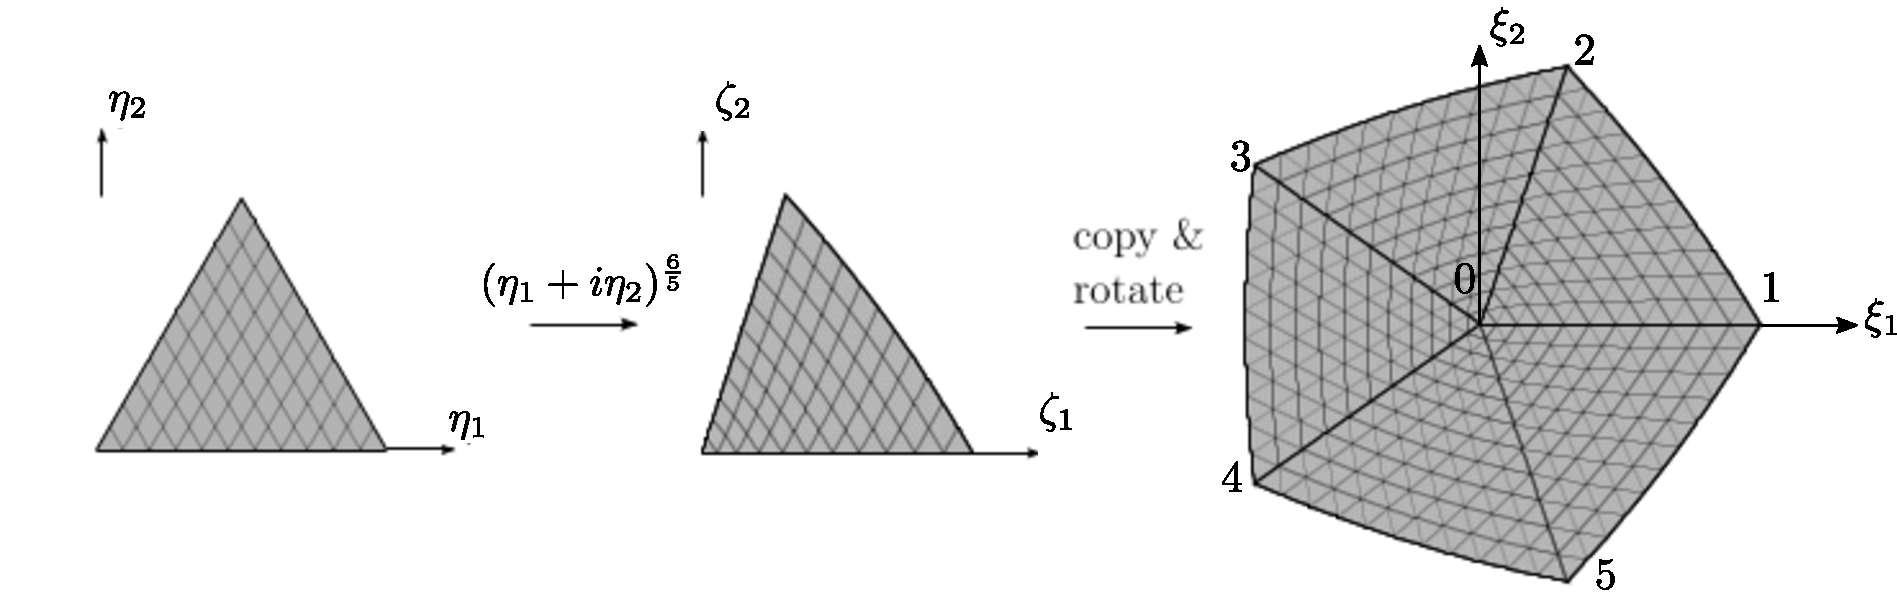
\includegraphics[scale=0.4]{figs/q1.pdf}
\end{center}
\begin{enumerate}[label=(\alph*)]
\item Calculate the coordinates of the 6 points on the patch.

\textbf{Solution}

The transformation in question is a non-linear transformation. This is evident from that fact that \textbf{$f(u+v) \neq f(u) + f(v)$}. Graphically, this is also evident as the grid-lines of the coordinates are not parallel and evenly spaced after our transformation.

The transformation takes points from the unit square on the real plane to the imaginary plane as given by 

\begin{equation*}
    \vec \zeta = f(\eta_1, \eta_2) = (\eta_1 + i\eta_2)^{\frac{6}{5}}
\end{equation*}


To find the coordinates of the patch, we first find the angle $\alpha$ as indicated in the following diagram:

\begin{center}
  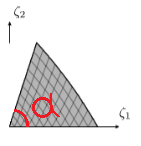
\includegraphics[scale=0.75]{alpha.png}
\end{center}

After calculating $\alpha$, we apply the transformation matrix, given by:

\begin{equation*}
\mat{R}=
\begin{bmatrix} 
       cos(\alpha) & -sin(\alpha)\\
       sin(\alpha) & cos(\alpha)\\
\end{bmatrix}   
\end{equation*}

This matrix is applied to transformed points on the unit triangle. The transformed points are the original points:\footnote{The point $(\eta_1, \eta_2) = (0.5, \sqrt{0.75})$ is calculated by using the Pythagorean theorem on the unit triangle.}
\begin{center}
$(0,0), (0,1),
(0.5, \sqrt{0.75})$
\end{center}
 on the unit triangle as given by the transformation $\vec \zeta$.

The following code was implemented in \textbf{MATLAB}, which explains the procedure for calculating the 6 points:

\begin{verbatim}
n0 = [0; 0]; %Point 0 of unit triangle
n1 = [1; 0]; %Point 1 of unit triangle
n2 = [0.5; sqrt(0.75)]; %Point 2 of unit triangle
alpha = angle((n2(1,1)+1i*n2(2,1))^(6/5))
%Angle between point 1 and point 2 in radians
P1 = complex_power(n0) %Point 0
P1 = complex_power(n1) %Point 1
P2 = complex_power(n2) %Point 2
P3 = rotation(P2, alpha) %Point 3
P4 = rotation(P3, alpha) %Point 4
P5 = rotation(P4, alpha) %Point 5
function y = complex_power(x) %complex power function
y = (x(1,1)+1i*x(2,1))^(6/5);
y = [real(y); (imag(y))];
end
function y = rotation(x, alpha) %rotation matrix function
R = [cos(alpha), -sin(alpha); sin(alpha), cos(alpha)];
y = R*x;
end
\end{verbatim}

Thus, after implementing the code as indicated above, we obtain the following coordinates $(\xi_{1}, \xi_{2})$ for the transformed points:

\begin{center}
    P0 = (0, 0\textit{i})\\
    P1 = (1, 0\textit{i})\\
    P2 = (0.3090, 0.9511\textit{i})\\
    P3 = (-0.8090, 0.5878\textit{i})\\
    P4 = (-0.8090, -0.5878\textit{i})\\
    P5 = (0.3090, -0.9511\textit{i})\\
\end{center}



\item An engineer measured the charge distribution $q$ on the 6 points of the patch as follows:
    \begin{center}
    \begin{tabular}{ | l | l | l | l | l | l | l |}
    \hline
    Point \# & 0 & 1 & 2 & 3 & 4 & 5  \\ \hline
    q        & 1 & 3 & 1 & 0 & 1 & 2 \\ \hline
    \end{tabular}
    \end{center}
    An electrical engineer is interested in finding out the charge $q$ at $\vec \xi = (0.5, 0.5)^T$. He also tells you that the charge inside the patch can be approximated using a bilinear polynomial $(1, \xi_1, \xi_2,\xi_1\xi_2)$. Compute $q$ at $\vec \xi = (0.5, 0.5)^T$.
    
    \textbf{Solution}
    
    To obtain the best polynomial approximation for the coordinates provided to us in the table above, we need to calculate the values of the coefficients of the bilinear polynomial described above. The polynomial is:

    \begin{center}
        $ P(\xi_{1}, \xi_{2}) = a + b\xi_{1} + c\xi_{2} + d\xi{1}\xi_{2} $
    \end{center}

    The above system is over-determined, as we have only 4 unknowns in the bilinear polynomial but 6 data points to be fitted. To find the solution, we must solve for $\mat{A}\vec{x} = \vec{b}$. The matrix $\mat{A}$ will be a $6 \times 4$ matrix:
    
    \begin{equation*}
        A = \begin{bmatrix}
               1 & 0 & 0 & 0 \\
               1 & 1 & 0 & 0 \\
               1 & 0.3090 & 0.9511 & (0.3090 \times 0.9511) \\
               1 & -0.8090 & 0.5878 & (-0.8090 \times 0.5878) \\
               1 & -0.8090 & -0.5878 & (-0.8090 \times -0.5878) \\
                1 & 0.3090 & -0.9511 & (0.3090 \times -0.9511) \\
        \end{bmatrix}
    \end{equation*}
    
    We also have $\vec{b} = \begin{bmatrix}
           1 \\
           3 \\
           1 \\
           0 \\
           1 \\
           2 \\
    \end{bmatrix}$.
    
    Solving for $\vec{x}$, we thus obtain the following vector:
    
    \begin{center}
        $\vec{x} = \begin{bmatrix}
            1.3333 \\
            1.2472 \\
            -0.6155 \\
            0.2906 \\
        \end{bmatrix}$
    \end{center}
    
    We thus end up with the following bilinear polynomial:
    
    \begin{center}
        $ P(\xi_{1}, \xi_{2}) = 1.3333 + 1.2472\xi_{1} -0.6155\xi_{2} + 0.2906\xi{1}\xi_{2} $
    \end{center}
    
    Computing $q$ at $\vec \xi = (0.5, 0.5)^T$:
    
    \begin{center}
        $ P(0.5, 0.5) = 1.3333 + 1.2472(0.5) -0.6155(0.5) + 0.2906(0.5)^{2} $
    \end{center}
    \begin{center}
        $ P(0.5, 0.5) = 1.7218$
    \end{center}
    
    Therefore, the value of $q$ at the point $(0.5, 0.5)$ is 1.7218.
    
    \item Sketch the charge distribution surface over the $\xi_{1} - \xi_{2}$ patch.
\end{enumerate}

\textbf{Solution}

    The figure was plotted in \textbf{MATLAB} using the following code:
    
    \begin{verbatim}
        figure
fmesh(@(x,y) 1.3333 + 1.2472.*x -0.6155.*y + 0.2906.*x.*y,
[-10 10 -10 10])
    \end{verbatim}
    
    \begin{center}
        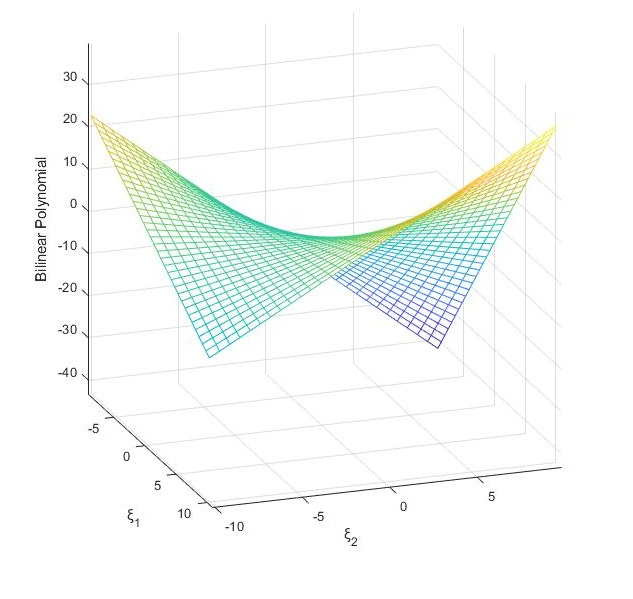
\includegraphics[scale=0.75]{q6.jpg}
    \end{center}

\item We have learned that for underdetermined systems, it is impossible to find unique solutions in the absence of some extra constraints. One way of obtaining the unique solution is to impose a minimum $L_2$ norm constraint i.e.
\begin{align}
\text{Solve: } \;\; \mat A \vec x &= \vec b \\
\text{such that: } \;\; \|\vec x\|_2 &\;\; \text{is minimum}
\end{align}
In this case, $\vec x_r = \mat A^T (\mat A \mat A^T)^{-1} \vec b$. By way of example explain the relationship between $\vec x_p$ and $\vec x_n$, and when $\vec x_p = \vec x_r$. Sketch the four fundamental subspaces.

\textbf{Solution}

Underdetermined systems correspond to wide matrices, i.e. Matrices with more equations than unknowns. One such matrix is the following matrix:

\begin{center}
    $\mat{A} = \begin{bmatrix}
           1 & 0 & 2 & 0 \\
           0 & 1 & 0 & 2
    \end{bmatrix}$
\end{center}

The matrix $\mat{A}$ above is in $\mat{RREF}$.

The free variables in the matrix above are $x_3$ and $x_4$. To find the special solutions, we first set $x_3 = 1$ and $x_4 = 0$.

This gives us the special solution $s_1 = \begin{bmatrix}
       0 \\
       -2 \\
       0 \\
       1 \\
\end{bmatrix}$.

Similarly, we now set $x_3 = 0$ and $x_4 = 1$.

\item Explain, with reason, whether the following statements are true or false

\begin{enumerate}[label=(\alph*)]
\item The complete solution is any linear combination of $x_p$ and $x_n$
\begin{itemize}
    \item 
    This statement is false because $x_p$ can not be any vector whereas $x_n$ can be any constant multiplied by the vector
\end{itemize}
\item A system $\mat A \vec x = \vec b$ has at most one particular solution
\begin{itemize}
    \item
    This statement is false as $\mat A \vec x = \vec b$ can have more than one particular solutions.
    One counterexample: If $x_p$ is one particular solution, and  $x_n$ $\in$ $N( \mat A) $, then $x_p$+ $x_n$ is also a particular solution.
\end{itemize}
\item The solution $x_p$ with all free variables set to zero can be the shortest solution (minimum length $\|x\|$)

\begin{itemize}
    \item
    Setting free variables to zero, doesn't mean getting the shortest solution
    Take    $ A = \begin{bmatrix}
    1 & 1 \\ 3 & 3
    \end{bmatrix}$
    and $ b  = \begin{bmatrix}
    2  \\ 0
    \end{bmatrix}$
    The free variable is $x_2$
    \\ 
    \\
    Setting $x_2 = 0$ and $x_1=2$\\
    So, $x_p =\begin{bmatrix}
    2  \\ 0
    \end{bmatrix}$
    while length of $x_p = 4$
    \newline        Setting $x_2 = 1 $ and $x_1=1$\\
    So, $x_p =\begin{bmatrix}
    1 \\ 1
    \end{bmatrix}$
    while length of $x_p = \sqrt{2}$
    
    which shows that setting free variables to zero does not guarantee shortest solution.
    

    
\end{itemize}
\item If $\mat A$ is invertible there is no solution $x_n$ in the nullspace
\begin{itemize}
    \item
   There is always the zero vector in the nullspace. So, $x_n = 0$ always exists. Thus false.
\end{itemize}
\end{enumerate}

\item True or false (with a reason or a counterexample)
\begin{enumerate}[label=(\alph*)]
\item $\mat A$ and $\mat A^T$ have the same number of pivots
\begin{itemize}
    \item \textbf{TRUE} A matrix and its transpose have the same rank as since transposition interchanges rows and columns, and a matrix always has same column and row rank which most essentially means that number of pivot variables which is also seen as the rank of the matrix, must stay the same.
\end{itemize}
\item $\mat A$ and $\mat A^T$ have the same left nullspace.
\begin{itemize}
    \item \textbf{FALSE}  If we take a 1x2 matrix, such as A =
    $\begin{bmatrix}
    1 & 1
    \end{bmatrix}$
The left nullspace of A contains vectors in R while the left nullspace of $A^T$, which
is the right nullspace of A, contains vectors in $R^2$
, so they cannot be the same.
\end{itemize}

\item If the row space equals the column space then $\mat A = \mat A^T$
\begin{itemize}
    \item \textbf{FALSE}. Counterexample: $ A = \begin{bmatrix}
    1 & 2 \\ 3 & 4
    \end{bmatrix}$
    Here, row space and column space equals $R^2$ as A  is invertible, but $A\neq A^T$
\end{itemize}
\item If $-\mat A = \mat A^T$, then the row space of $\mat A$ equals the column space 
\begin{itemize}
    \item \textbf{TRUE}
    The null spaces are identical because $Ax = 0 =$  ($-$ $A)x = 0.$
The column spaces are identical because any vector v that can be expressed
as $v = Ax$ for some x can also be expressed as $v = (−A)(−x)$. A similar
reasoning holds for the two remaining subspaces. The row space of A is equal to the column space of $A^T$ which for this A equals the column space of -A. Since, A and -A have same fundamental subspaces, we can conclude that row space of A equals the column space of A.
    
\end{itemize}
\end{enumerate}



\item For the space $\mathbb R^4$, let $w_1 = \begin{bmatrix} 1 \\ 1 \\ 1 \\ 1\end{bmatrix}, w_2 = \begin{bmatrix} 3 \\ 3 \\ -1 \\ -1\end{bmatrix}, y = \begin{bmatrix} 6 \\ 0 \\ 2 \\ 0\end{bmatrix}$, and let $W = \text{sp}\{w_1, w_2\}$. 

\begin{enumerate}[label=(\alph*)]
\item Find a basis for $W$ consisting of two orthogonal vectors using Gram-Schmidt process.
\item Explain the Gram-Schmidt process intuitively. 
\item Express $y$ as the sum of a vector in $W$ and a vector in $W^\perp$
\end{enumerate}

Please refer to \MYhref{https://textbooks.math.gatech.edu/ila/orthogonal-sets.html}{this link} for this question

\end{enumerate}

\newpage

\section*{Appendix A: Code for Q2}
\begin{verbatim}
import matplotlib.pyplot as plt 
import numpy as np

x = [i for i in np.arange(-10, 10, 0.1)]

def basis_1(x):
	return x**2 - 49
def basis_2(x):
	return x - 7

b1 = [basis_1(i) for i in x]
b2 = [basis_2(i) for i in x]

fig = plt.figure()
basis = fig.add_subplot(111)
basis.set_xlabel('x')
basis.set_title("basis for p(7) = 0")

basis.plot(x, b1, label=f'x\N{SUPERSCRIPT TWO} - 49')
basis.plot(x, b2, label='x - 7')
basis.plot(x, [-49 for i in x], linestyle='--', label='y = -49')
basis.set_title('Basis Functions for p(7) = 0')

basis.grid(linestyle='-')
legend = basis.legend()
plt.show()

\end{verbatim}

\newpage

\begin{thebibliography}{}
    \bibitem{formatting} 
    Formatting Python strings with super script for Q2.
    \begin{verbatim}
    https://stackoverflow.com/questions/8651361/
        how-do-you-print-superscript-in-python/49442772
    \end{verbatim}
    
    \bibitem{matplotlib} 
    Plotting Basis with matplotlib
    \begin{verbatim}
    https://matplotlib.org/3.1.0/gallery/pyplots/fig_axes_labels_simple.html
    \end{verbatim}

\end{thebibliography}{}
\end{document}
